%==============================================================================
%  Informe del Proyecto Final
%  Procesamiento de Imagenes y Vision Computacional, UCB "San Pablo"
%  Compilar con pdfLaTeX.
%==============================================================================
\documentclass[10pt,a4paper]{article}
\usepackage[utf8]{inputenc}
\usepackage[T1]{fontenc}
\usepackage[spanish,es-tabla]{babel}
\usepackage{lmodern}
\usepackage{microtype}
\usepackage[top=1.9cm,bottom=1.9cm,left=1.8cm,right=1.8cm]{geometry}
\usepackage{titlesec}
\usepackage{graphicx}
\usepackage{booktabs}
\usepackage{amsmath,amssymb}
\usepackage{xcolor}
\usepackage{caption}
\usepackage{subcaption}
\usepackage{enumitem}
\usepackage{float}
\usepackage{array}
\usepackage[hidelinks]{hyperref}

\captionsetup{font=small,labelfont=bf,skip=3pt}
\setlist{itemsep=0.5pt,topsep=2pt,parsep=0pt}
\titlespacing*{\section}{0pt}{7pt plus 1pt minus 1pt}{3pt}
\titlespacing*{\subsection}{0pt}{5pt plus 1pt minus 1pt}{2pt}
\titleformat{\section}{\large\bfseries}{\thesection}{0.6em}{}
\titleformat{\subsection}{\normalsize\bfseries}{\thesubsection}{0.5em}{}
\setlength{\textfloatsep}{7pt plus 2pt minus 2pt}
\setlength{\intextsep}{7pt plus 2pt minus 2pt}
\setlength{\abovedisplayskip}{4pt}
\setlength{\belowdisplayskip}{4pt}
\setlength{\parskip}{0pt}
\renewcommand{\arraystretch}{1.05}
\setlength{\emergencystretch}{1em}

\newcommand{\tituloproyecto}{Sistema de Visión Computacional para la\\ Detección de Comercio Informal en la Vía Pública}
\newcommand{\subtituloproyecto}{Transfer learning secuencial COCO $\rightarrow$ KITTI $\rightarrow$ Santa Cruz con YOLO11n}
\newcommand{\integranteA}{Ana Patricia Aban Monzon}
\newcommand{\integranteB}{Juan Pablo Meriles}
\newcommand{\docente}{Erick Antero Maraz Zu\~niga}
\newcommand{\repositorio}{https://github.com/patyaban/Deteccion-Comercio-Informal-SCZ}

\begin{document}

%============================== PORTADA =======================================
\begin{titlepage}
\centering

\includegraphics[width=0.24\textwidth]{ucb-logo.png}\\[0.9cm]
{\large Universidad Católica Boliviana ``San Pablo''}\\[0.2cm]
{\large Sede Santa Cruz de la Sierra}\\[1.1cm]
{\normalsize Diplomado en Inteligencia Artificial}\\[0.2cm]
{\normalsize Módulo: Procesamiento de Imágenes y Visión Computacional}\\[1.4cm]
\rule{\textwidth}{0.7pt}\\[0.5cm]
{\LARGE\bfseries \tituloproyecto\par}
\vspace{0.4cm}
{\large \subtituloproyecto\par}
\rule{\textwidth}{0.7pt}\\[1.4cm]
{\large\bfseries Integrantes}\\[0.3cm]
{\large \integranteA}\\[0.15cm]
{\large \integranteB}\\[1.2cm]
{\large\bfseries Docente}\\[0.3cm]
{\large \docente}\\[1.4cm]
{\large Santa Cruz de la Sierra, Bolivia, agosto de 2026}
\vfill
{\footnotesize\textbf{Repositorio del proyecto:} \url{\repositorio}\\
código, notebooks, pesos e instrucciones de reproducción.}
\end{titlepage}

%============================== 1. RESUMEN ====================================
\section{Resumen}
Las vías públicas de Santa Cruz de la Sierra concentran una alta densidad de puestos y
vendedores en acera y calzada, cuyo registro se realiza hoy mediante inspección manual.
Este proyecto entrena un detector de objetos capaz de localizar, sobre fotografías
tomadas a nivel de calle, tres elementos del comercio en vía pública: puestos o
estructuras (\texttt{street\_stall}), vendedores (\texttt{street\_vendor}) y personas
sentadas (\texttt{person\_sitting}). A ellos se suman seis clases de contexto vial y
peatonal.
Se construyó un conjunto propio de 220 imágenes anotadas y se comparó, con
hiperparámetros idénticos, una arquitectura YOLO11n entrenada desde cero contra la misma
arquitectura sometida a \emph{transfer learning} secuencial en dos etapas: una adaptación
de dominio vial sobre KITTI a partir de pesos COCO, y luego una especialización sobre el
conjunto local con el \emph{backbone} congelado (\texttt{freeze=10}). Sobre el conjunto de
prueba, la estrategia secuencial alcanzó \textbf{mAP@0.5 = 0{,}4164} frente a
\textbf{0{,}1430} del modelo desde cero, con un \emph{recall} de 0{,}4227 contra 0{,}1312.
Con un conjunto de datos de este tamaño, el resultado depende más de la transferencia de
representaciones que de la arquitectura o del número de épocas, y el modelo obtenido es
utilizable como asistente de pre-etiquetado, no como sistema de medición autónomo.

%========================= 2. INTRODUCCIÓN ====================================
\section{Introducción y motivación}
\textbf{Problema.} Dada una fotografía tomada a la altura de un peatón en una calle de
Santa Cruz de la Sierra, localizar con una caja delimitadora cada puesto, toldo, mesa o
carretilla instalado en la vía pública, cada persona que atiende esos puestos, y los
elementos de tráfico y flujo peatonal que los rodean. La salida es una lista de cajas con
clase y confianza, no una etiqueta única por imagen.

\textbf{Caso real análogo.} Es el mismo problema que resuelven los sistemas de
\emph{street-level imagery analytics} de empresas como Mapillary o Numina para
inventariar mobiliario urbano: un vehículo recorre la vía y un detector convierte el
video en un inventario georreferenciado. La diferencia está en el catálogo de clases, que
no existe en los \emph{datasets} públicos de conducción autónoma.

\textbf{Por qué importa.} El uso previsto no es el conteo automático definitivo sino el
\textbf{pre-etiquetado} (\emph{auto-labeling}): una unidad municipal de catastro que deba
construir un registro de ocupación de vía pública anota hoy miles de imágenes a mano, y un
detector con \emph{recall} razonable convierte esa tarea en una de revisión y corrección
de cajas propuestas. La decisión que alimenta es logística: qué tramos priorizar en un
relevamiento. El sistema se limita a describir la ocupación observable del espacio y no
clasifica situaciones como regulares o irregulares.

%============================== 3. DATOS ======================================
\section{Datos}
\subsection{Fuentes y esquema de clases}
Se emplearon dos conjuntos con roles distintos. \textbf{KITTI} \cite{kitti}, en la
distribución de Ultralytics \cite{ultralytics}, aporta la etapa intermedia: 7{.}481
imágenes de escena vial ($\approx$5{.}985 de entrenamiento y 1{.}496 de validación) con 8
clases viales, bajo licencia CC BY-NC-SA 3.0 y descarga automática al ejecutar
\texttt{src/train.py}. El \textbf{conjunto propio de Santa Cruz} aporta la etapa final:
220 fotografías capturadas con teléfono móvil en agosto de 2026 en vías con actividad
comercial de la ciudad, anotadas manualmente por el equipo con LabelImg \cite{labelimg} y
exportadas a formato YOLO (\texttt{clase cx cy w h}, normalizado); son de autoría propia,
sin licencia de terceros involucrada.

Se definieron 9 clases. Las seis primeras, \texttt{car} (0), \texttt{van} (1),
\texttt{truck} (2), \texttt{pedestrian} (3), \texttt{person\_sitting} (4) y
\texttt{cyclist} (5), conservan deliberadamente los índices y la semántica de KITTI, de
modo que la etapa intermedia sea informativa para ellas. Las tres últimas,
\texttt{street\_vendor} (6), \texttt{street\_stall} (7) y \texttt{motorbike} (8), son
propias del dominio.

\subsection{Partición y balance}
La partición es 70/20/10 sobre la lista de pares imagen-anotación, ordenada
alfabéticamente y barajada con semilla fija (\texttt{random.Random(0)}): 154 imágenes de
entrenamiento, 44 de validación y 22 de prueba. Es una partición \emph{aleatoria por
imagen}, no estratificada por clase; con 220 imágenes y 9 categorías una estratificación
real no es viable, y la consecuencia se observa en la Tabla~\ref{tab:balance}:
\texttt{cyclist} no aparece en el conjunto de prueba y \texttt{van} lo hace con 2
instancias.

\begin{table}[H]
\centering\footnotesize
\caption{Distribución de cajas delimitadoras por clase y partición.}
\label{tab:balance}
\begin{tabular}{@{}lrrrrrrrrrrr@{}}
\toprule
\textbf{Partición} & \texttt{car} & \texttt{van} & \texttt{truck} & \texttt{pedest.} &
\texttt{p\_sitting} & \texttt{cyclist} & \texttt{vendor} & \texttt{stall} & \texttt{moto} &
\textbf{Cajas} & \textbf{Imág.}\\
\midrule
Entrenamiento & 96 & 23 & 17 & 422 & 50 & 6 & 124 & 368 & 41 & \textbf{1.147} & 154\\
Validación    & 30 &  3 & 12 & 125 & 27 & 2 &  32 & 106 & 10 & \textbf{347}   &  44\\
Prueba        & 12 &  2 &  3 &  67 &  6 & 0 &  24 &  53 &  6 & \textbf{173}   &  22\\
\midrule
\% del entrenamiento & 8{,}37 & 2{,}01 & 1{,}48 & 36{,}79 & 4{,}36 & 0{,}52 & 10{,}81 &
32{,}08 & 3{,}57 & 100{,}00 & \\
\bottomrule
\end{tabular}\\[2pt]
{\scriptsize Abreviaturas: \texttt{pedest.}\,=\,\texttt{pedestrian},
\texttt{p\_sitting}\,=\,\texttt{person\_sitting}, \texttt{vendor}\,=\,\texttt{street\_vendor},
\texttt{stall}\,=\,\texttt{street\_stall}, \texttt{moto}\,=\,\texttt{motorbike}.}
\end{table}

\subsection{Limitaciones conocidas del conjunto de datos}
\begin{enumerate}[leftmargin=*]
  \item \textbf{Tamaño.} 220 imágenes y 1{.}667 cajas en total. Con 173 instancias en
        prueba, cada objeto no detectado mueve el \emph{recall} global en $\approx$0{,}6
        puntos: las métricas reportadas tienen un intervalo de confianza amplio.
  \item \textbf{Riesgo de fuga por grupo.} Las fotografías se tomaron el mismo día y en
        pocos tramos de calle, de modo que varias imágenes comparten el mismo puesto
        visto desde ángulos distintos. Como la partición es aleatoria por imagen y no por
        escena, un mismo puesto físico puede aparecer en entrenamiento y en prueba, lo
        que infla las métricas respecto de calles no vistas.
  \item \textbf{Desbalance severo.} \texttt{pedestrian} y \texttt{street\_stall}
        concentran el 68{,}9\,\% de las cajas de entrenamiento, mientras \texttt{cyclist}
        aporta 6 cajas y \texttt{truck} 17: las clases minoritarias no tienen soporte
        estadístico suficiente para una evaluación seria.
  \item \textbf{Sesgo de captura y ambigüedad de anotación.} Todas las fotos son diurnas,
        con buena luz y tomadas a la altura del pecho desde la vereda opuesta. Además, la
        frontera entre \texttt{street\_vendor} y \texttt{pedestrian}, es decir entre
        quien atiende y quien compra, es una decisión de criterio que dos anotadores no
        aplican de forma perfectamente consistente.
  \item \textbf{Un archivo corrupto.} Una imagen de prueba está truncada y Ultralytics
        la descarta automáticamente: la evaluación se realiza sobre 21 imágenes.
\end{enumerate}

%============================ 4. METODOLOGÍA ==================================
\section{Metodología}
\subsection{Arquitectura y justificación}
Se usó \textbf{YOLO11n} \cite{yolo11,ultralytics}: 2{.}583{.}907 parámetros y 6{,}4
GFLOPs. La elección responde a tres razones concretas del proyecto y no a una preferencia
general. Primero, con 154 imágenes de entrenamiento un modelo de mayor capacidad memoriza
el conjunto en pocas épocas, y la variante \emph{nano} es la que mejor se ajusta a este
régimen de datos. Segundo, el uso previsto, que es el pre-etiquetado por lotes y,
eventualmente, el procesamiento de video, exige inferencia barata: el modelo ejecuta en 19{,}2\,ms por
imagen sobre la GPU de entrenamiento y en \textbf{313\,ms en CPU}, sin dependencia de
CUDA, de modo que revisar un lote de imágenes no requiere GPU. Tercero, existe un
\emph{checkpoint} COCO \cite{coco} oficial de esta misma arquitectura, requisito para la
primera etapa de transferencia.

\subsection{Estrategia de transferencia secuencial y modelo de control}
La hipótesis del experimento es que la distancia entre COCO (objetos genéricos, encuadres
variados) y el dominio final (calle de Santa Cruz, perspectiva peatonal, oclusión densa)
es demasiado grande para un salto único, y que una etapa intermedia en un dominio vial
reduce ese desajuste \cite{yosinski}:
\[
\underbrace{\text{COCO}}_{\text{pesos generales}}
\ \xrightarrow[\text{10 épocas, backbone libre}]{\textbf{Etapa 1}}\
\underbrace{\text{KITTI}}_{\text{dominio vial}}
\ \xrightarrow[\text{80 épocas, \texttt{freeze=10}}]{\textbf{Etapa 2}}\
\underbrace{\text{Santa Cruz}}_{\text{comercio en vía pública}}
\]
En la Etapa 2 el \emph{head} de detección se reinicializa automáticamente al cambiar el
número de clases ($nc$: $8 \rightarrow 9$) y se congelan las 10 primeras capas, es decir el
\emph{backbone} completo hasta el bloque C2PSA, de modo que el entrenamiento sobre las
154 imágenes locales solo ajusta el cuello y la cabeza de detección; esto evita que un
conjunto pequeño destruya los extractores de características ya aprendidos. Para que la
comparación sea atribuible a la transferencia, el modelo de control parte de
\texttt{yolo11n.yaml} (pesos aleatorios) con exactamente los mismos datos, épocas, tamaño
de imagen, \emph{batch}, optimizador, aumentaciones y semilla: la única diferencia entre
ambas ramas es el punto de partida de los pesos y el congelamiento.

\subsection{Preprocesamiento y aumentación}
Las imágenes se redimensionan a $640\times640$ con relleno. La conversión de coordenadas
de Pascal VOC a YOLO, con el centro y las dimensiones normalizados por el ancho y el alto
de la imagen, se implementó explícitamente y se verifica con una aserción en
\texttt{src/preparar\_datos.py}. Se usaron las aumentaciones por defecto de Ultralytics,
idénticas en ambas ramas: mosaico ($p=1{,}0$, desactivado en las últimas 10 épocas),
volteo horizontal ($p=0{,}5$), variación HSV ($h=0{,}015$; $s=0{,}7$; $v=0{,}4$), escala
$\pm0{,}5$, traslación $\pm0{,}1$ y borrado aleatorio ($p=0{,}4$). No se aplicó volteo
vertical ni rotación: la perspectiva de calle tiene una orientación vertical fija.

\subsection{Hiperparámetros}
Los valores de la Tabla~\ref{tab:hp} son los \emph{defaults} de \texttt{argparse} en
\texttt{src/train.py}, de modo que ejecutar el script sin argumentos reproduce el
resultado reportado. No se realizó barrido de hiperparámetros, porque no había presupuesto
de cómputo ni un conjunto de validación lo bastante grande para que resultara
significativo. Los valores provienen del laboratorio de la Sesión 10 del curso, con
dos ajustes deliberados, 80 épocas en lugar de 30 (con 10 iteraciones por época la curva
de validación seguía subiendo) y \texttt{freeze=10} por el argumento anterior.

\begin{table}[H]
\centering\footnotesize
\caption{Hiperparámetros. Las dos ramas comparten todo salvo el origen de los pesos.}
\label{tab:hp}
\begin{tabular}{@{}lccc@{}}
\toprule
& \textbf{Etapa 1 (KITTI)} & \textbf{Etapa 2 (SCZ, \emph{transfer})} & \textbf{Control (desde cero)}\\
\midrule
Pesos iniciales & \texttt{yolo11n.pt} (COCO) & \texttt{best.pt} de Etapa 1 & aleatorios\\
Épocas / \texttt{freeze} & 10 / sin congelar & 80 / 10 & 80 / sin congelar\\
Tamaño de imagen / \emph{batch} & 640 / 16 & 640 / 16 & 640 / 16\\
Optimizador & SGD & SGD & SGD\\
LR inicial / final & 0{,}01 / 0{,}0001 & 0{,}01 / 0{,}0001 & 0{,}01 / 0{,}0001\\
\emph{Momentum} / \emph{decay} & 0{,}937 / 0{,}0005 & 0{,}937 / 0{,}0005 & 0{,}937 / 0{,}0005\\
Semilla & 0 & 0 & 0\\
Tiempo (Tesla T4) & 18{,}0 min & 12{,}7 min & 13{,}5 min\\
\bottomrule
\end{tabular}
\end{table}

%============================= 5. RESULTADOS ==================================
\section{Resultados}
\subsection{Etapa intermedia y comparación en el conjunto de prueba}
Tras 10 épocas sobre KITTI el modelo alcanzó mAP@0.5 = 0{,}607 y mAP@0.5:0.95 = 0{,}371
sobre las 1{.}496 imágenes de validación, con \texttt{car} en 0{,}888 y
\texttt{person\_sitting} en 0{,}356 como extremos. El valor absoluto no es el objetivo,
porque 10 épocas están lejos de agotar KITTI. Lo relevante es que estos pesos ya codifican
la perspectiva y la escala de una escena de calle antes de ver una imagen de Santa Cruz.

\begin{table}[H]
\centering\footnotesize
\begin{minipage}[t]{0.395\textwidth}
\centering
\caption{Métricas globales sobre el conjunto de prueba (21 imágenes, 173 instancias).}
\label{tab:test}
\begin{tabular}{@{}lccc@{}}
\toprule
\textbf{Métrica} & \textbf{Desde cero} & \textbf{TL sec.} & \textbf{Factor}\\
\midrule
mAP@0.5      & 0{,}1430 & \textbf{0{,}4164} & $\times$2{,}91\\
mAP@0.5:0.95 & 0{,}0483 & \textbf{0{,}2036} & $\times$4{,}22\\
Precisión (P)& \textbf{0{,}6224} & 0{,}4882 & $\times$0{,}78\\
\emph{Recall} (R) & 0{,}1312 & \textbf{0{,}4227} & $\times$3{,}22\\
\bottomrule
\end{tabular}
\end{minipage}\hfill
\begin{minipage}[t]{0.575\textwidth}
\centering\setlength{\tabcolsep}{4.5pt}
\caption{Desempeño por clase del modelo secuencial en prueba. La clase \texttt{cyclist}
no tiene instancias en este conjunto.}
\label{tab:clases}
\begin{tabular}{@{}lrrrrr@{}}
\toprule
\textbf{Clase} & \textbf{Inst.} & \textbf{P} & \textbf{R} & \textbf{mAP@0.5} & \textbf{mAP@0.5:0.95}\\
\midrule
\texttt{truck}          &  3 & 0{,}928 & 0{,}667 & 0{,}717 & 0{,}387\\
\texttt{car}            & 12 & 0{,}519 & 0{,}667 & 0{,}572 & 0{,}345\\
\texttt{street\_stall}  & 53 & 0{,}527 & 0{,}604 & 0{,}552 & 0{,}209\\
\texttt{pedestrian}     & 67 & 0{,}669 & 0{,}403 & 0{,}525 & 0{,}253\\
\texttt{motorbike}      &  6 & 0{,}604 & 0{,}500 & 0{,}479 & 0{,}172\\
\texttt{street\_vendor} & 24 & 0{,}413 & 0{,}375 & 0{,}394 & 0{,}214\\
\texttt{person\_sitting}&  6 & 0{,}246 & 0{,}167 & 0{,}093 & 0{,}048\\
\texttt{van}            &  2 & 0{,}000 & 0{,}000 & 0{,}000 & 0{,}000\\
\midrule
\textbf{Global} & \textbf{173} & 0{,}488 & 0{,}423 & \textbf{0{,}416} & \textbf{0{,}204}\\
\bottomrule
\end{tabular}
\end{minipage}
\end{table}

La precisión más alta del modelo desde cero es un artefacto y no una ventaja: con un
\emph{recall} de 0{,}13 emite muy pocas detecciones y en varias clases (\texttt{truck},
\texttt{motorbike}, \texttt{person\_sitting}) registra precisión 1{,}000 con
\emph{recall} 0{,}000, es decir, un puñado de detecciones aisladas sobre un fondo de
omisiones. En una herramienta de pre-etiquetado el \emph{recall} es la métrica que decide
la utilidad: corregir una caja sobrante cuesta un clic, encontrar un objeto omitido
cuesta releer la imagen completa.

Las dos clases centrales del problema se comportan de forma distinta.
\texttt{street\_stall}, con 53 instancias, es la mejor sostenida: recupera 6 de cada 10
puestos con precisión 0{,}527, suficiente para usarlo como propuesta de anotación.
\texttt{street\_vendor} se queda en 0{,}394 por una razón previsible: un vendedor es
visualmente un peatón, y lo que lo distingue es su relación espacial con la mercadería,
una señal contextual que un detector de una etapa entrenado con 124 ejemplos no llega a
modelar. Los valores de \texttt{van} (0{,}000) y \texttt{person\_sitting} (0{,}093) no
son un fracaso del modelo: con 2 y 6 instancias, una sola omisión colapsa la métrica.

\subsection{Curvas de aprendizaje}
\begin{figure}[H]
\centering
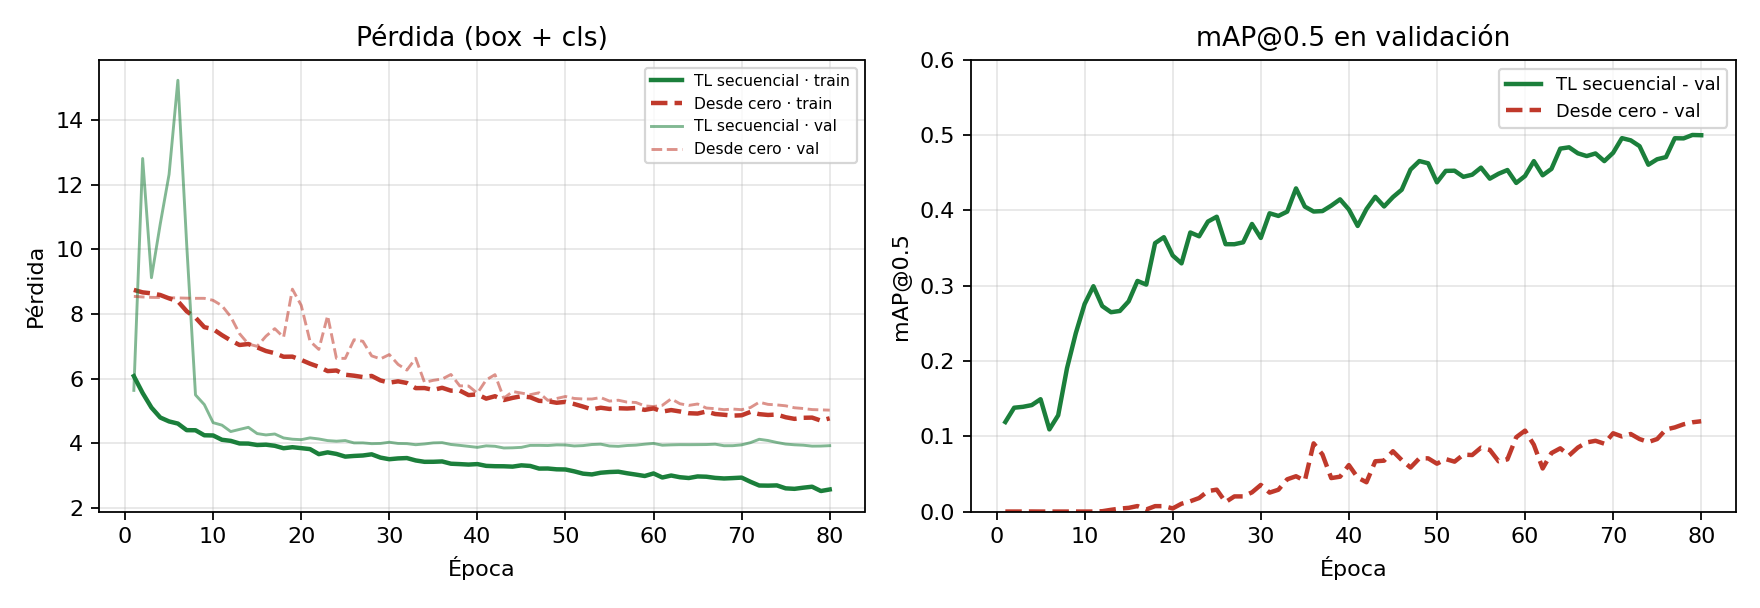
\includegraphics[width=0.66\textwidth]{figuras/curvas_train_val.png}
\caption{Izquierda: pérdida (\texttt{box\_loss} + \texttt{cls\_loss}) de entrenamiento en
trazo grueso y de validación en trazo claro. Derecha: mAP@0.5 sobre el conjunto de
validación, por época. Ambas ramas comparten hiperparámetros y semilla.}
\label{fig:curvas}
\end{figure}

La Figura~\ref{fig:curvas} contiene los hallazgos más informativos del experimento. La
rama transferida arranca en una pérdida de entrenamiento de 6{,}08 mientras la rama desde
cero arranca en 8{,}74, y esa brecha nunca se cierra: en la época 80 la primera está en
2{,}57 y la segunda en 4{,}77, valor que la rama transferida ya había superado en la
época 5. En validación, la rama transferida llega a 0{,}299 de mAP@0.5 en la época 11,
mientras que la rama desde cero permanece por debajo de 0{,}01 durante las primeras 15
épocas y termina en 0{,}120. Los picos de la pérdida de validación al comienzo
corresponden al calentamiento del \emph{learning rate}, no a inestabilidad del modelo.

Las dos ramas están, sin embargo, en regímenes opuestos. En la rama transferida la
pérdida de validación toca su mínimo en la \textbf{época 43} (3{,}854) y luego se estanca
y remonta levemente hasta 3{,}926, mientras la de entrenamiento sigue cayendo: la brecha
entre ambas pasa de $+0{,}52$ en la época 40 a $+1{,}36$ en la 80. Eso es sobreajuste
incipiente y, con 154 imágenes, era esperable. Lo llamativo es que el mAP@0.5 de
validación \emph{sigue subiendo} en ese tramo, hasta 0{,}500 en la época 79: el modelo
empeora la calibración de sus confianzas, que es lo que castiga la pérdida, mientras
continúa afinando la localización y el ordenamiento de las detecciones, que es lo que mide
el mAP. La rama desde cero no muestra nada de eso: su pérdida de validación todavía caía
en la época 80 y la brecha con entrenamiento es de apenas $+0{,}25$. Está sencillamente
\textbf{subentrenada}.

\subsection{Análisis cualitativo}
\begin{figure}[H]
\centering
\begin{subfigure}{0.385\textwidth}
  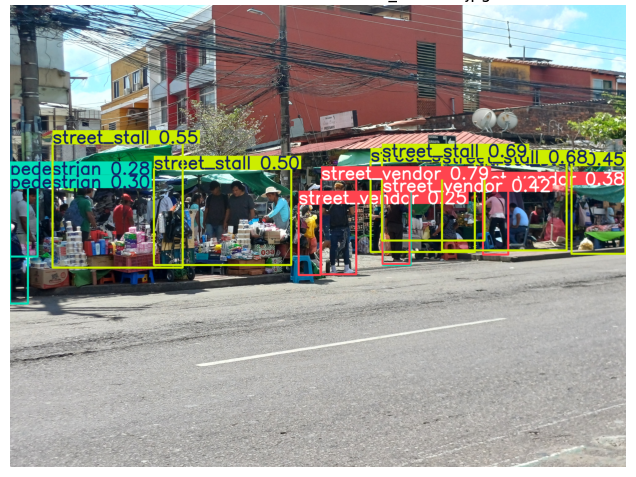
\includegraphics[width=\textwidth]{figuras/prediccion_1.png}
  \caption{Fila de puestos con toldos sobre la acera.}
\end{subfigure}\hspace{0.025\textwidth}%
\begin{subfigure}{0.212\textwidth}
  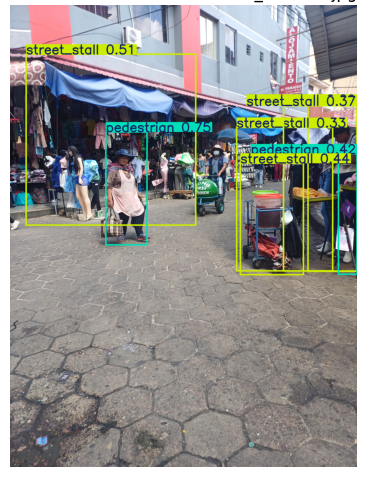
\includegraphics[width=\textwidth]{figuras/prediccion_2.png}
  \caption{Escena con oclusión.}
\end{subfigure}
\caption{Predicciones del modelo secuencial sobre imágenes del conjunto de prueba, con
umbral de confianza 0{,}25.}
\label{fig:preds}
\end{figure}

En la Figura~\ref{fig:preds}(a) el modelo delimita seis estructuras contiguas bajo
toldos, con confianzas entre 0{,}38 y 0{,}69, y distingue a cuatro vendedores dentro de
esa fila; en la Figura~\ref{fig:preds}(b), sobre una escena más ocluida, recupera el
peatón en primer plano con confianza 0{,}75 y cuatro puestos al fondo, pero omite parte
de las personas del segundo plano. Para cuantificar los modos de falla se emparejaron
predicciones y anotaciones por IoU sobre 16 fotografías, con 186 casos resultantes:
51{,}1\,\% de aciertos, 25{,}8\,\% de omisiones, 14{,}0\,\% de falsos positivos y
7{,}5\,\% de confusiones de clase. Más de la mitad de los errores se concentra en tres
mecanismos: personas y puestos ocluidos en escenas densas (25 casos), detecciones espurias
de baja confianza (15) y puestos contiguos que el NMS suprime por solapamiento mutuo (11).
Los ejemplos individuales, doce aciertos y doce fallos, están en la
Figura~\ref{fig:errores} y el desglose completo en el Anexo~\ref{anexo:errores}.

%========================= 6. DISCUSIÓN =======================================
\section{Discusión y limitaciones}
\textbf{Lo que funcionó mejor de lo esperado.} La magnitud del efecto de la
transferencia: con 154 imágenes la expectativa razonable era una mejora de algunos puntos
y el resultado fue casi el triple de mAP@0.5. También resultó llamativo que
\texttt{street\_stall}, una clase que no existe en COCO ni en KITTI y de apariencia muy
variable, quedara entre las mejor detectadas: los filtros heredados responden a la
geometría de toldos y estructuras rectangulares aunque nunca hayan visto esa categoría.

\textbf{Lo que no funcionó.} La separación \texttt{street\_vendor} /
\texttt{pedestrian} sigue siendo el cuello de botella, y es un problema de formulación
además de datos: son la misma clase visual diferenciada por contexto. La etapa intermedia
sobre KITTI, además, aporta menos de lo que promete para las clases nuevas, porque al
cambiar $nc$ de 8 a 9 el \emph{head} se reinicializa por completo y lo único que se
transfiere son \emph{backbone} y cuello. Por último, el umbral de confianza quedó mal
elegido: el 0{,}25 por defecto de Ultralytics genera 26 falsos positivos cada 95 aciertos,
y subirlo a 0{,}40 elimina el 73\,\% de ellos a cambio del 14\,\% de los aciertos
(Anexo~\ref{anexo:errores}).

\textbf{Señales de sobreajuste.} Las hay, y solo en la rama transferida
(Figura~\ref{fig:curvas}): el modelo empieza a memorizar el conjunto de 154 imágenes a
partir de la época 43. La lectura práctica es que había margen para detener el
entrenamiento antes: con \texttt{patience} en torno a 15 épocas se habría obtenido un
modelo equivalente en la mitad del tiempo. Aun así, el \emph{checkpoint} final sigue siendo
el mejor de la corrida, porque el mAP nunca deja de mejorar. La rama desde cero no
da ninguna señal de sobreajuste: se detuvo por presupuesto de épocas, no por
convergencia.

\textbf{Fuga de datos y sesgos.} El riesgo de fuga por grupo es la limitación
metodológica más seria y está presente: la partición es aleatoria por imagen sobre
fotografías tomadas el mismo día en pocos tramos de calle, de modo que un mismo puesto
puede estar en entrenamiento y en prueba visto desde otro ángulo. La corrección adecuada
es una partición por escena o por cuadra, que exige registrar esa metadata al capturar;
mientras no se haga, el 0{,}4164 reportado debe leerse como una cota superior optimista.
A ello se suman el sesgo de captura, con tomas diurnas, de buen clima y desde una
distancia y altura similares, y un sesgo geográfico: las zonas fotografiadas son las
accesibles al equipo, no una muestra representativa de la ciudad.

\textbf{Uso responsable.} El sistema describe la presencia y ubicación de elementos
observables en la vía pública. No identifica personas, ya que no se aplicó reconocimiento
facial, ni infiere condición legal alguna de la actividad detectada, y su salida no
constituye evidencia suficiente para ninguna acción administrativa individual.

%======================== 7. TRABAJO FUTURO ===================================
\section{Trabajo futuro}
\begin{enumerate}[leftmargin=*]
  \item \textbf{Repartición por escena y captura de metadata.} Registrar coordenada GPS y
        tramo de calle en cada fotografía y rehacer la partición agrupando por cuadra, de
        modo que ningún puesto físico aparezca en dos particiones. No mejorará la métrica,
        probablemente la reduzca, pero es la única forma de conocer el desempeño real.
  \item \textbf{Incorporar el conjunto \emph{street-level} de vendedores informales}
        \cite{streetlevel} ($\approx$1{.}400 imágenes anotadas, CC BY 4.0) como tercera
        etapa intermedia entre KITTI y Santa Cruz: aportaría dos órdenes de magnitud más
        de ejemplos de \texttt{street\_vendor}, hoy la clase más débil.
  \item \textbf{Ampliar la captura a franja vespertina y nocturna.} Las horas de mayor
        actividad comercial están sub-representadas en el conjunto actual, enteramente
        diurno; se necesitan al menos 100 imágenes con iluminación artificial y contraluz.
  \item \textbf{Reformular \texttt{street\_vendor} como relación y no como clase.}
        Detectar \texttt{pedestrian} y \texttt{street\_stall} por separado y derivar la
        condición de vendedor de la proximidad y el solapamiento entre ambas cajas, en
        lugar de pedirle al detector que distinga dos siluetas humanas idénticas.
\end{enumerate}

%========================== 8. CONCLUSIONES ===================================
\section{Conclusiones}
Con 220 imágenes propias y una arquitectura de 2{,}6 millones de parámetros, el
\emph{transfer learning} secuencial COCO $\rightarrow$ KITTI $\rightarrow$ Santa Cruz con
\emph{backbone} congelado alcanzó mAP@0.5 = 0{,}4164 en prueba frente a 0{,}1430 del mismo
modelo entrenado desde cero bajo hiperparámetros idénticos, con un \emph{recall} 3{,}2
veces mayor: en un régimen de datos escaso, el punto de partida de los pesos pesa más que
cualquier otro factor bajo control del equipo. El modelo resultante sirve como asistente
de pre-etiquetado, ya que detecta seis de cada diez puestos en 313\,ms por imagen y sin
GPU, pero no como sistema de medición autónomo, y su desempeño es una cota superior
optimista mientras la partición no se realice por escena. El código, los pesos y las
instrucciones de reproducción están en \url{\repositorio}.

%========================== 9. REFERENCIAS ====================================
\begin{thebibliography}{9}\scriptsize
\setlength{\itemsep}{1pt}\setlength{\parskip}{0pt}
\bibitem{yolo11} R.~Khanam y M.~Hussain, ``YOLOv11: An Overview of the Key Architectural
Enhancements,'' \emph{arXiv preprint} arXiv:2410.17725, 2024.
\bibitem{ultralytics} G.~Jocher, J.~Qiu y A.~Chaurasia, ``Ultralytics YOLO11,'' 2024.
\url{https://github.com/ultralytics/ultralytics}. Licencia AGPL-3.0.
\bibitem{kitti} A.~Geiger, P.~Lenz y R.~Urtasun, ``Are we ready for Autonomous Driving?
The KITTI Vision Benchmark Suite,'' en \emph{IEEE CVPR}, 2012, pp.~3354--3361.
\bibitem{coco} T.-Y.~Lin \emph{et al.}, ``Microsoft COCO: Common Objects in Context,'' en
\emph{ECCV}, 2014, pp.~740--755.
\bibitem{yosinski} J.~Yosinski, J.~Clune, Y.~Bengio y H.~Lipson, ``How transferable are
features in deep neural networks?,'' en \emph{NeurIPS}, 2014, pp.~3320--3328.
\bibitem{streetlevel} D.~García-Jaimes \emph{et al.}, ``Street-level imagery dataset for
the detection of informal vendors in urban environments,'' \emph{Data in Brief}, 2025.
\url{https://doi.org/10.5281/zenodo.14635548}. Licencia CC BY 4.0.
\bibitem{labelimg} Tzutalin, ``LabelImg: Graphical image annotation tool,'' 2015.
\url{https://github.com/HumanSignal/labelImg}. Licencia MIT.
\end{thebibliography}

%============================== ANEXO =========================================
\appendix
\section{Anexo: análisis de errores}
\label{anexo:errores}
Sobre 16 fotografías anotadas del conjunto propio, con umbral de confianza 0{,}25 e IoU de
emparejamiento 0{,}5, se analizaron 186 casos: 95 aciertos (51{,}1\,\%), 48 omisiones
(25{,}8\,\%), 26 falsos positivos (14{,}0\,\%), 14 confusiones de clase (7{,}5\,\%) y 3
detecciones duplicadas (1{,}6\,\%). La Figura~\ref{fig:errores} muestra doce aciertos y
doce fallos representativos, y la Tabla~\ref{tab:modos} agrupa los 91 errores por
mecanismo. El detalle caso por caso, con las 186 filas y su clase predicha, la clase real,
la confianza, el IoU y una hipótesis, está en
\texttt{resultados/analisis/analisis\_errores.xlsx} del repositorio.
\begin{table}[H]
\centering\scriptsize
\caption{Modos de falla observados, ordenados por frecuencia.}
\label{tab:modos}
\begin{tabular}{@{}p{3.9cm}r p{11.4cm}@{}}
\toprule
\textbf{Modo} & \textbf{N} & \textbf{Hipótesis}\\
\midrule
Omisión en escena densa & 25 & Personas y puestos ocluidos entre sí o al fondo, con pocos píxeles: \texttt{pedestrian} (15) y \texttt{street\_vendor} (10).\\
Omisión en fila de puestos & 11 & Sin frontera visual entre un puesto y el siguiente, el NMS suprime las cajas intermedias por solapamiento con la del vecino.\\
Omisión de clases minoritarias & 12 & \texttt{motorbike} (5), \texttt{person\_sitting} (3), \texttt{truck} (2), \texttt{car} (1) y \texttt{cyclist} (1), casi siempre ocluidos tras puestos y con soporte escaso en el conjunto local.\\
Caja mal encuadrada & 11 & Falsos positivos con IoU entre 0{,}2 y 0{,}5: el objeto existe, el recuadro no calza; no son invenciones del modelo.\\
Detección espuria & 15 & Falsos positivos con IoU $\leq$ 0{,}2, sobre textura de mercadería y toldos; 18 de los 26 falsos positivos quedan por debajo de 0{,}35 de confianza.\\
Confusión \texttt{pedestrian} $\leftrightarrow$ \texttt{street\_vendor} & 6 & Misma silueta humana; lo que las separa es la relación espacial con la mercadería, contexto que un detector de una etapa no modela.\\
Otras confusiones de clase & 8 & \texttt{person\_sitting} y \texttt{cyclist} (4) no tienen soporte para discriminar postura; carretillas y triciclos de venta comparten estructura con \texttt{motorbike} y \texttt{truck} (2); \texttt{van} frente a \texttt{truck} es una frontera ambigua heredada de KITTI (2).\\
Detección duplicada & 3 & Dos cajas sobre el mismo objeto con solapamiento por debajo del umbral de NMS de 0{,}7.\\
\midrule
\textbf{Total} & \textbf{91} & \\
\bottomrule
\end{tabular}
\end{table}

\noindent\textbf{Elección del umbral de confianza.} Los falsos positivos tienen confianza
media 0{,}350 frente a 0{,}646 de los aciertos, y 18 de los 26 caen por debajo de 0{,}35.
Reevaluar los mismos 186 casos variando el umbral (Tabla~\ref{tab:umbral}) muestra que el
0{,}25 por defecto de Ultralytics no es el adecuado para esta tarea: subirlo a 0{,}40
elimina el 73\,\% de los falsos positivos y el 59\,\% de las confusiones y duplicados a
cambio del 14\,\% de los aciertos, y eleva la precisión de 68{,}8\,\% a 85{,}4\,\%. Para el
pre-etiquetado conviene en principio un umbral bajo, pero con 26 falsos positivos cada 95
aciertos revisar deja de ser más rápido que anotar: 0{,}40 es el compromiso razonable con
este modelo.

\begin{table}[H]
\centering\footnotesize
\caption{Efecto del umbral de confianza sobre los 186 casos analizados.}
\label{tab:umbral}
\begin{tabular}{@{}lccccc@{}}
\toprule
\textbf{Umbral} & \textbf{0{,}25 (usado)} & \textbf{0{,}30} & \textbf{0{,}35} & \textbf{0{,}40} & \textbf{0{,}50}\\
\midrule
Aciertos          & 95 & 92 & 84 & \textbf{82} & 71\\
Falsos positivos  & 26 & 16 &  8 & \textbf{7}  &  2\\
Confusiones y duplicados & 17 & 14 & 12 & \textbf{7} & 5\\
Precisión         & 68{,}8\,\% & 75{,}4\,\% & 80{,}8\,\% & \textbf{85{,}4\,\%} & 91{,}0\,\%\\
\bottomrule
\end{tabular}
\end{table}

\begin{figure}[H]
\centering

\includegraphics[width=\textwidth]{figuras/analisis_errores.png}
\caption{Doce aciertos (arriba) y doce fallos (abajo) del modelo secuencial sobre imágenes
anotadas del conjunto propio, con umbral de confianza 0{,}25. En los aciertos se indica la
clase predicha y su confianza; en los fallos, el tipo de error: clase equivocada, objeto
anotado no detectado o falso positivo.}
\label{fig:errores}
\end{figure}

\end{document}
